% Options for packages loaded elsewhere
\PassOptionsToPackage{unicode}{hyperref}
\PassOptionsToPackage{hyphens}{url}
%
\documentclass[
  11pt,
]{article}
\usepackage{amsmath,amssymb}
\usepackage{lmodern}
\usepackage{iftex}
\ifPDFTeX
  \usepackage[T1]{fontenc}
  \usepackage[utf8]{inputenc}
  \usepackage{textcomp} % provide euro and other symbols
\else % if luatex or xetex
  \usepackage{unicode-math}
  \defaultfontfeatures{Scale=MatchLowercase}
  \defaultfontfeatures[\rmfamily]{Ligatures=TeX,Scale=1}
  \setmainfont[]{Times New Roman}
\fi
% Use upquote if available, for straight quotes in verbatim environments
\IfFileExists{upquote.sty}{\usepackage{upquote}}{}
\IfFileExists{microtype.sty}{% use microtype if available
  \usepackage[]{microtype}
  \UseMicrotypeSet[protrusion]{basicmath} % disable protrusion for tt fonts
}{}
\makeatletter
\@ifundefined{KOMAClassName}{% if non-KOMA class
  \IfFileExists{parskip.sty}{%
    \usepackage{parskip}
  }{% else
    \setlength{\parindent}{0pt}
    \setlength{\parskip}{6pt plus 2pt minus 1pt}}
}{% if KOMA class
  \KOMAoptions{parskip=half}}
\makeatother
\usepackage{xcolor}
\usepackage[margin=1.0in]{geometry}
\usepackage{graphicx}
\makeatletter
\def\maxwidth{\ifdim\Gin@nat@width>\linewidth\linewidth\else\Gin@nat@width\fi}
\def\maxheight{\ifdim\Gin@nat@height>\textheight\textheight\else\Gin@nat@height\fi}
\makeatother
% Scale images if necessary, so that they will not overflow the page
% margins by default, and it is still possible to overwrite the defaults
% using explicit options in \includegraphics[width, height, ...]{}
\setkeys{Gin}{width=\maxwidth,height=\maxheight,keepaspectratio}
% Set default figure placement to htbp
\makeatletter
\def\fps@figure{htbp}
\makeatother
\setlength{\emergencystretch}{3em} % prevent overfull lines
\providecommand{\tightlist}{%
  \setlength{\itemsep}{0pt}\setlength{\parskip}{0pt}}
\setcounter{secnumdepth}{5}
\newcommand{\bcenter}{\begin{center}}
\newcommand{\ecenter}{\end{center}}
\newcommand{\btitlepage}{\begin{titlepage}}
\newcommand{\etitlepage}{\end{titlepage}}
\usepackage{setspace}\onehalfspacing
\usepackage{booktabs}
\usepackage[font=small,labelfont=bf]{caption}
\usepackage{booktabs}
\usepackage{longtable}
\usepackage{array}
\usepackage{multirow}
\usepackage{wrapfig}
\usepackage{float}
\usepackage{colortbl}
\usepackage{pdflscape}
\usepackage{tabu}
\usepackage{threeparttable}
\usepackage{threeparttablex}
\usepackage[normalem]{ulem}
\usepackage{makecell}
\usepackage{xcolor}
\ifLuaTeX
  \usepackage{selnolig}  % disable illegal ligatures
\fi
\IfFileExists{bookmark.sty}{\usepackage{bookmark}}{\usepackage{hyperref}}
\IfFileExists{xurl.sty}{\usepackage{xurl}}{} % add URL line breaks if available
\urlstyle{same} % disable monospaced font for URLs
\hypersetup{
  hidelinks,
  pdfcreator={LaTeX via pandoc}}

\author{}
\date{\vspace{-2.5em}}

\begin{document}

\begin{titlepage}

\begin{center}

\vspace*{30mm}

Candidate number: 49045

\vspace*{5mm}

\hypertarget{replication-of-hansen-2015-punishment-and-deterrence-evidence-from-drunk-driving}{%
\section*{Replication of Hansen (2015) Punishment and Deterrence:
Evidence from Drunk
Driving}\label{replication-of-hansen-2015-punishment-and-deterrence-evidence-from-drunk-driving}}
\addcontentsline{toc}{section}{Replication of Hansen (2015) Punishment
and Deterrence: Evidence from Drunk Driving}

\vspace*{30mm}

Submitted as the summative assessment for\\

PB4A7: Quantitative Applications for Behavioural Science 2022

\end{center}

\end{titlepage}

\newpage

In the study \emph{Punishment and Deterrence: Evidence from Drunk
Driving} \textbf{(Hansen, 2015)}, Hansen investigated the effect of
punishments and sanctions on reducing repeat drunk driving. The study
implemented a quasi-experimental design, utilising the administrative
records from 1995 to 2011 of the state of Washington, U.S., where two
thresholds of blood alcohol content (BAC) are used to determine the
status of driving under the influence (DUI). Specifically, a driver with
a measured BAC over 0.08 is considered a case of DUI and will be
punished via measures such as fines, jail time, and driving license
suspension. One with a BAC over 0.15 is considered a case of aggravated
DUI, to which more severe punishments and sanctions are applied. Since
BAC measure has clear-cut numeric thresholds for determining whether a
driver will receive harsher punishments, and neither drivers or police
can manipulate this measure, Hansen applied a regression discontinuity
design to analyse the data \textbf{(expand on the justification of using
RDD)}. He hypothesized that receiving harsher punishments and sanctions
at both thresholds would reduce offenders' future recidivism of DUI. He
further applied the RDD to analyse the effect of receiving harsher
punishments on the degree of deterrence, incapacitation, and
rehabilitation in order to identify the mechanism through which harsher
punishments might reduce recidivism \textbf{(check the paper to see
whether this sentence is precise)}.

\textbf{Ideally also the results}

The present study aims to replicate the findings from \textbf{Hansen
(2015)} using regression discontinuity design applied to a similar data
\textbf{(what is it exactly\ldots)}. It will be focused on estimating
the effect of receiving punishments on reducing recidivism at the 0.08
BAC threshold only. The paper proceeds as follows. Section 1 discusses
the econometric method and assumptions underlying its application to the
current data. Section 2 presents the main results, and Section 3
discusses critiques and extensions to the original study. Section 4
concludes.

\hypertarget{methods-and-assumptions}{%
\section{Methods and Assumptions}\label{methods-and-assumptions}}

\hypertarget{assumptions-of-the-regression-discontinuity-design}{%
\subsection{Assumptions of the regression discontinuity
design}\label{assumptions-of-the-regression-discontinuity-design}}

The present study applies the regression discontinuity design to the
data provided by the class instructor. Several assumptions need to be
met so that the regression discontinuity design can give accurate
estimates. First, people need to be randomly assigned to receiving
punishment at the BAC threshold. In other words, neither the drivers nor
the police can manipulate the BAC level and thus whether one will
receive punishment. \textbf{Hansen (2015)} has already given a plausible
theoretical justification for this assumption. Empirically, I plot the
distribution of BAC and test for discontinuity in its distribution at
the threshold. Figure \ref{fig:bac_hist_continuous} shows the
distribution of BAC level. Based on a recently developed local
polynomial density estimator \textbf{(CJM, 2020)}, the hypothesis that
the distribution is continuous at 0.08 cannot be rejected at the alpha
level of 0.05 (\emph{p} = 0.890). Therefore, there is no evidence for
the existence of manipulation on the BAC level.

\begin{figure}[H]
  \centering
  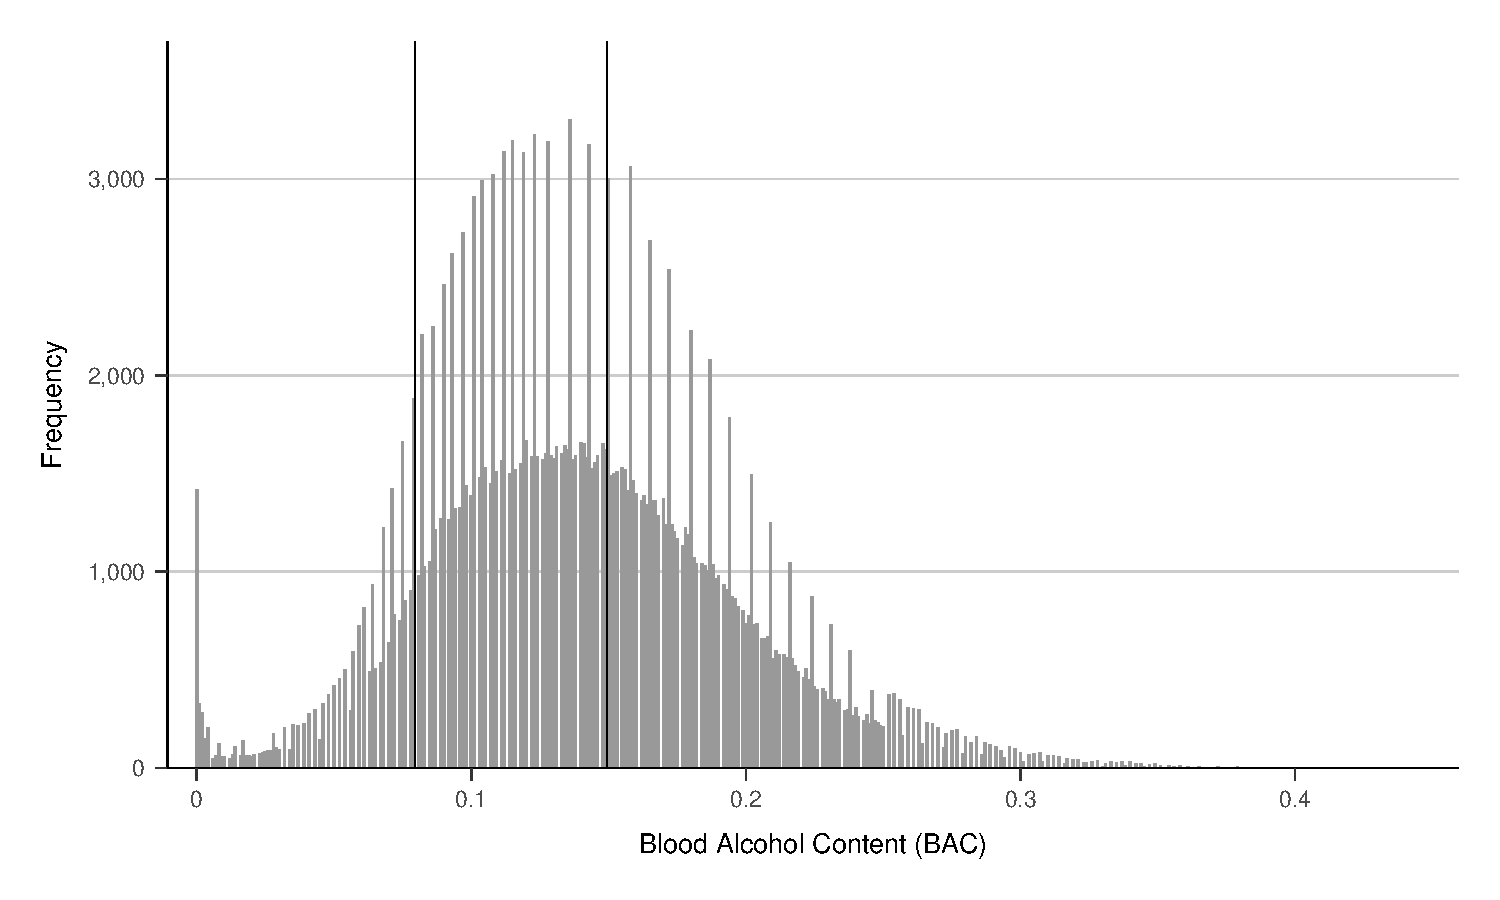
\includegraphics[width=0.9\columnwidth]{../figures/bac_histogram_continuous.pdf}
  \caption{\textbf{Histogram of blood alcohol content as a continuous variable.} The blood alcohol content is plotted as a continuous variable with a bin width of 0.001, the precision used on the breathalysers. The y-axis represents the frequency of observations in each bin. The vertical black lines represent the two thresholds at 0.08 and 0.15.}
  \label{fig:bac_hist_continuous}
\end{figure}

The second assumption is that the running variable should not contain
non-random heaping, which can lead to biased estimates in regression
discontinuity models \textbf{(Barreca et al., 2011)}. In other words,
BAC should not be much more likely to take certain values than others.
Based on Figure \ref{fig:bac_hist_continuous}, this assumption seems to
be violated. Curiously, when BAC is plotted as a discrete variable,
non-random heaping disappears (Figure \ref{fig:bac_hist_discrete}). A
closer inspection of the data suggests that this is probably due to the
lack of precision in BAC in the current data. Many BAC values deviate by
a very small amount from the values that are supposed to be given by the
breathalysers (i.e., precise to three digits after the decimal point).
Some bins have a value at the left boundary deviating upwards and a
value at the right boundary deviating downwards. Such bins will contain
a larger number of observations than other bins and thus leads to
heaping. This would not occur if the data records the values precisely
so that the number of observations are rightly separated into and
plotted by two bins, or if we treat BAC as discrete and give each value
its own bin. \textbf{(consider using a simulation to justify this
claim?)}

\begin{figure}[H]
  \centering
  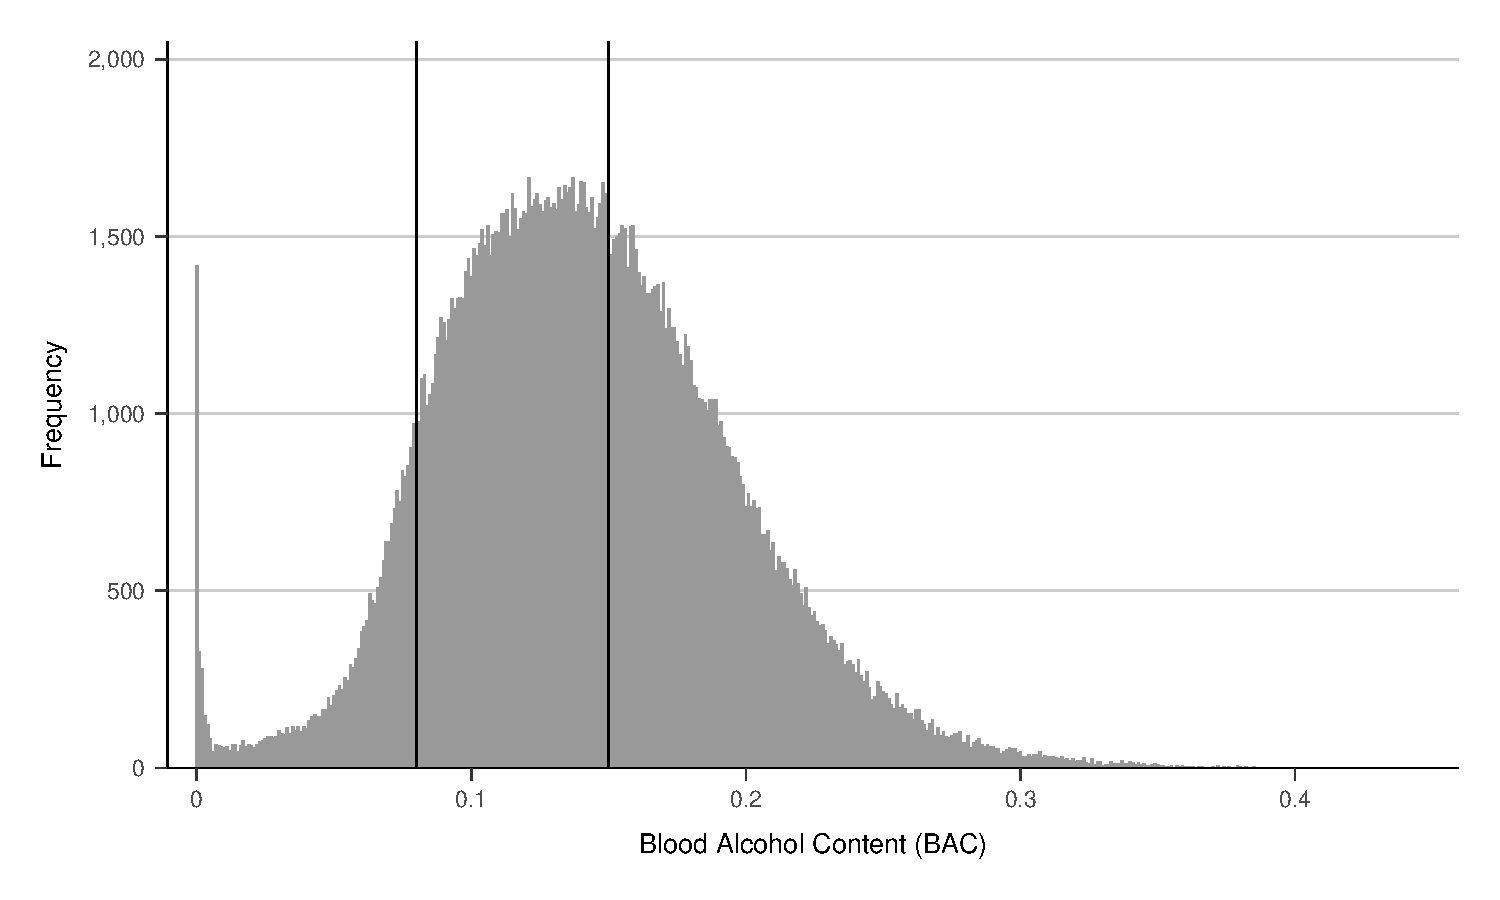
\includegraphics[width=0.9\columnwidth]{../figures/bac_histogram_discrete.pdf}
  \caption{\textbf{Histogram of blood alcohol content as a discrete variable.} The blood alcohol content is plotted as a discrete variable with a bin width of 0.001, the precision used on the breathalysers. The y-axis represents the frequency of observations in each bin. The vertical black lines represent the two thresholds at 0.08 and 0.15.}
  \label{fig:bac_hist_discrete}
\end{figure}

\hypertarget{the-model}{%
\subsection{The model}\label{the-model}}

The present study utilises a local linear regression model with a
rectangular kernel weight function to estimate the effect of receiving
punishments at the threshold on recidivism. For sensitivity analyses,
the models are re-estimated using second-order polynomials and triangle
kernel function). The model is specified by the following function:

\begin{equation}
  \label{eqn:model}
  R_i = \alpha + \beta_1 DUI_i + \beta_2 BAC_i + \beta_3 DUI_i \times BAC_i + \tau Z_i + \epsilon_i
\end{equation}

where the variable \(DUI_i\) is an indicator of whether BAC is above the
0.08 threshold, \(BAC_i\) is the measure of BAC level, \(R_i\) is an
indicator of recidivism, and \(Z_i\) is a vector of control variables.
The variable \(BAC_i\) in the model is centered around the threshold
value of 0.08 so that the coefficients directly reflect the estimates of
the effect.

\hypertarget{inclusion-of-control-variables}{%
\subsection{Inclusion of control
variables}\label{inclusion-of-control-variables}}

In order to determine whether any covariates should be included in the
model, I run preliminary analyses on the effect of receiving punishments
at the threshold on four predetermined characteristics, including three
demographic variables (gender, race, and age) and the BAC test being
conducted in a traffic accident. The analyses use the same local linear
regression model specified in equation (\ref{eqn:model}), with a
bandwidth of 0.05 and no kernel weight function. As Table
\ref{tab:covariate} shows, I fail to reject any of the null hypotheses
that predetermined characteristics remained the same at the threshold.
This indicates that gender, race, age, and the BAC test being conducted
in a traffic accident, on average, were not different between people who
did not receive punishments and those who received punishments at the
threshold. According to \textbf{Calonico et al.~(2019)}, I will include
the four predetermined characteristics in regression discontinuity
models to improve the estimation precision of the effects of receiving
punishments at the threshold on recidivism.

\begingroup
\renewcommand{\arraystretch}{1.3}

\begin{table}

\caption{Regression Discontinuity Estimates of the Effect of Receiving Punishments at the 0.08 BAC Threshold on Predetermined Characteristics}
\label{tab:covariate}
\centering
\begin{threeparttable}
\begin{tabular}[t]{l>{\centering\arraybackslash}p{5em}>{\centering\arraybackslash}p{5em}>{\centering\arraybackslash}p{5em}>{\centering\arraybackslash}p{5em}}
\toprule
  & Male & White & Age & Accident\\
\midrule
\textit{DUI} & 0.006 & 0.006 & –0.141 & –0.003\\
 & (0.006) & (0.005) & (0.164) & (0.004)\\
Mean & 0.784 & 0.846 & 0.085 & 33.99\\
Num. of Obs. & 89,967 & 89,967 & 89,967 & 89,967\\
\bottomrule
\end{tabular}
\begin{tablenotes}
\small
\item \textit{Note.} Regression discontinuity based estimates of the effect of receiving punishments at the 0.08 BAC threshold on four predetermined characteristics. All models use a bandwidth of 0.05 and a rectangular kernel weight function. Counterfactual predictions of mean recidivism is calculated at the 0.079 BAC threshold. Heteroscedasticity-robust standard errors are in parentheses. $^{*}\, p<0.1$, $^{**}\, p<0.05$, $^{***}\, p<0.01$.
\end{tablenotes}
\end{threeparttable}
\end{table}

\endgroup

\hypertarget{results}{%
\section{Results}\label{results}}

\hypertarget{the-effect-of-punishments-on-recidivism}{%
\subsection{The Effect of Punishments on
Recidivism}\label{the-effect-of-punishments-on-recidivism}}

Table \ref{tab:main} reports the estimated effect of receiving
punishments at the threshold on recidivism. Local linear regression
model with a rectangular kernel function gives the estimate that
receiving punishments at the 0.08 BAC threshold decreases recidivism by
2.4 percentage points, which is statistically significant at the alpha
level of 0.01. Local second-order polynomial with a rectangular kernel
function gives an estimate of a decrease in recidivism by 1.4 percentage
points, which is statistically significant at the alpha level of 0.05.
These estimates are consistent across both bandwidths and across models
with different types of kernel functions.

\begingroup
\renewcommand{\arraystretch}{1.1}

\begin{table}

\caption{Regression Discontinuity Estimates of the Effect of Receiving Punishments at the 0.08 BAC Threshold on Recidivism}
\label{tab:main}
\centering
\begin{threeparttable}
\begin{tabular}[t]{l>{\centering\arraybackslash}p{8em}>{\centering\arraybackslash}p{8em}>{\centering\arraybackslash}p{8em}>{\centering\arraybackslash}p{8em}}
\toprule
\multicolumn{1}{c}{ } & \multicolumn{2}{c}{Rectangular kernel} & \multicolumn{2}{c}{Triangular kernel} \\
\cmidrule(l{3pt}r{3pt}){2-3} \cmidrule(l{3pt}r{3pt}){4-5}
  & Linear & Quadratic & Linear & Quadratic\\
\midrule
\multicolumn{5}{l}{\textit{DUI $\in$ [0.03, 0.13]}} \\
\textit{DUI} & –0.024*** & –0.014** & –0.020*** & –0.014**\\
 & (0.004) & (0.006) & (0.005) & (0.006)\\
Mean & 0.104 & 0.099 & 0.100 & 0.099\\
Controls & Yes & Yes & Yes & Yes\\
Num. of Obs. & 89,967 & 89,967 & 89,967 & 89,967\\
\addlinespace
\multicolumn{5}{l}{\textit{DUI $\in$ [0.055, 0.105]}} \\
\textit{DUI} & –0.021*** & –0.014* & –0.018*** & –0.016*\\
 & (0.006) & (0.008) & (0.006) & (0.009)\\
Mean & 0.101 & 0.098 & 0.101 & 0.100\\
Controls & Yes & Yes & Yes & Yes\\
Num. of Obs. & 46,957 & 46,957 & 46,957 & 46,957\\
\bottomrule
\end{tabular}
\begin{tablenotes}
\small
\item \textit{Note.} Regression discontinuity based estimates of the effect of receiving punishments at the 0.08 BAC threshold on recidivism. The upper panel presents estimates based on a 0.05 bandwidth, and the lower panel presents estimates based on a 0.025 bandwidth. The table includes results from both linear and quadratic models, with either a rectangular or a triangular kernel weight function. Controls include individuals' gender, race, age, and an indicator of whether the BAC test was conducted in a traffic accident. Counterfactual predictions of mean recidivism are calculated at the 0.079 BAC threshold and mean age of the respective populations, averaging over individuals' gender and race, as well as over whether the BAC testing was conducted in an accident. Heteroscedasticity-robust standard errors are in parentheses. $^{*}\, p<0.1$, $^{**}\, p<0.05$, $^{***}\, p<0.01$.
\end{tablenotes}
\end{threeparttable}
\end{table}

\endgroup

\hypertarget{robustness}{%
\subsection{Robustness}\label{robustness}}

Since there seems to be non-random heaping in the current data (Figure
\ref{fig:bac_hist_continuous}), this section will use donut regression
discontinuity models to investigate the robustness of the results
presented in the last section. Donut regression discontinuity models
entirely drop the observations near the threshold. Under appropriate
assumptions, they are effective in preventing a heap just at the
threshold from biasing the estimates \textbf{(Barreca et al., 2011)}.

For the present study, I drop the observations in the interval
\(BAC \in [0.079, 0.081]\), and re-estimate local linear regression and
quadratic models with either a rectangular or a triangular kernel weight
function. It is worth stressing that robustness test using local
polynomials is especially important in a donut regression discontinuity
design. This is because a donut regression model gets rid of the very
observations on which the estimates of local average effects rely upon.
The estimates given by donut regression models are essentially based on
models' extrapolation over the region of the donut \textbf{(Dowd, 2021)}
and may be especially sensitive to the assumptions about the underlying
functional form \textbf{(Consider justifying this using a simulation)}.
Using polynomials with different orders can ensure the robustness of the
results over different functional assumptions.

The results from donust regreesion discontinuity models are presented in
Table \ref{tab:donut}. According to the local linear regression model
with a rectangular kernel function, receiving punishments at the
threshold decreases recidivism by 2.6 percentage points and is
statistically significant at the alpha level of 0.01. According to the
local second-order polynomial with a rectangular kernel function,
receiving punishments at the threshold decreases recidivism by 1.4
percentage points and is statistically significant at the alpha level of
0.1. These estimates are consistent across both bandwidths and across
models with different types of kernel functions, except for not being
statistically significant in quadratic models estimated with narrower
bandwidth of 0.025. Therefore, the results given by donut regression
discontinuity models are essentially identical with those given by
ordinary models presents in the last section.

\begingroup
\renewcommand{\arraystretch}{1.1}

\begin{table}

\caption{Donut Regression Discontinuity Estimates of the Effect of Receiving Punishments at the 0.08 BAC Threshold on Recidivism}
\label{tab:donut}
\centering
\begin{threeparttable}
\begin{tabular}[t]{l>{\centering\arraybackslash}p{8em}>{\centering\arraybackslash}p{8em}>{\centering\arraybackslash}p{8em}>{\centering\arraybackslash}p{8em}}
\toprule
\multicolumn{1}{c}{ } & \multicolumn{2}{c}{Rectangular kernel} & \multicolumn{2}{c}{Triangular kernel} \\
\cmidrule(l{3pt}r{3pt}){2-3} \cmidrule(l{3pt}r{3pt}){4-5}
  & Linear & Quadratic & Linear & Quadratic\\
\midrule
\multicolumn{5}{l}{\textit{DUI $\in$ [0.03, 0.13]}} \\
\textit{DUI} & –0.026*** & –0.014* & –0.022*** & –0.018**\\
 & (0.005) & (0.007) & (0.005) & (0.006)\\
Mean & 0.105 & 0.099 & 0.102 & 0.101\\
Controls & Yes & Yes & Yes & Yes\\
Num. of Obs. & 88,085 & 88,085 & 88,085 & 88,085\\
\addlinespace
\multicolumn{5}{l}{\textit{DUI $\in$ [0.055, 0.105]}} \\
\textit{DUI} & –0.022*** & –0.015 & –0.020*** & –0.020\\
 & (0.007) & (0.011) & (0.007) & (0.012)\\
Mean & 0.103 & 0.099 & 0.103 & 0.104\\
Controls & Yes & Yes & Yes & Yes\\
Num. of Obs. & 45,075 & 45,075 & 45,075 & 45,075\\
\bottomrule
\end{tabular}
\begin{tablenotes}
\small
\item \textit{Note.} Regression discontinuity based estimates of the effect of receiving punishments at the 0.08 BAC threshold on recidivism after dropping observations in the interval [0.079, 0.081]. The upper panel presents estimates based on a 0.05 bandwidth, and the lower panel presents estimates based on a 0.025 bandwidth. The table includes results from both linear and quadratic models, with either a rectangular or a triangular kernel weight function. Controls include individuals' gender, race, age, and an indicator of whether the BAC test was conducted in a traffic accident. Counterfactual predictions of mean recidivism are calculated at the 0.079 BAC threshold and mean age of the respective populations, averaging over individuals' gender and race, as well as over whether the BAC testing was conducted in an accident. Heteroscedasticity-robust standard errors are in parentheses. $^{*}\, p<0.1$, $^{**}\, p<0.05$, $^{***}\, p<0.01$.
\end{tablenotes}
\end{threeparttable}
\end{table}

\endgroup

\hypertarget{discussion-critique-and-extension}{%
\section{Discussion, Critique and
Extension}\label{discussion-critique-and-extension}}

\hypertarget{conclusion}{%
\section{Conclusion}\label{conclusion}}

\end{document}
